\title{Hierarchical temporal framework for reinforcement learning: an end-to-end model of the brain}
\author{Aleksander Mendoza}

\documentclass[12pt]{article}
\usepackage{tikz}
\usepackage[utf8]{inputenc}
\usepackage[T1]{fontenc}
\usepackage{lmodern}
\usepackage{amsfonts}
\usepackage{mathrsfs}
\usepackage{centernot}
\usepackage{listings}
\usepackage{mathtools}
\usepackage{xcolor}
\usepackage{amsthm}
\usepackage{amsmath}
\usepackage{amssymb}
\usepackage{tikzit}
\usepackage{enumitem}
\input{style.tikzstyles}

\newtheorem{definition}{Definition}
\newtheorem{theorem}{Theorem}[section]
\newtheorem{corollary}{Corollary}[theorem]
\newtheorem{lemma}[theorem]{Lemma}
\renewcommand{\labelenumii}{\theenumii}
\renewcommand{\theenumii}{\theenumi.\arabic{enumii}.}
\begin{document}
\maketitle
\lstset{
	basicstyle=\ttfamily,
	mathescape
}


\begin{abstract}
	Reinforcement learning agent using end-to-end model of the brain based on HTM with voting, pattern separation,
	episodic memory and dopamine-like reward.
\end{abstract}

\tableofcontents

\section{Different perspective on reinforcement learning}

The model described here has been inspired by the observation that
reinforcement learning has a lot in common with spacial navigation (Figure \ref{fig:rl_problems}). 

\begin{figure}[!htbp]
	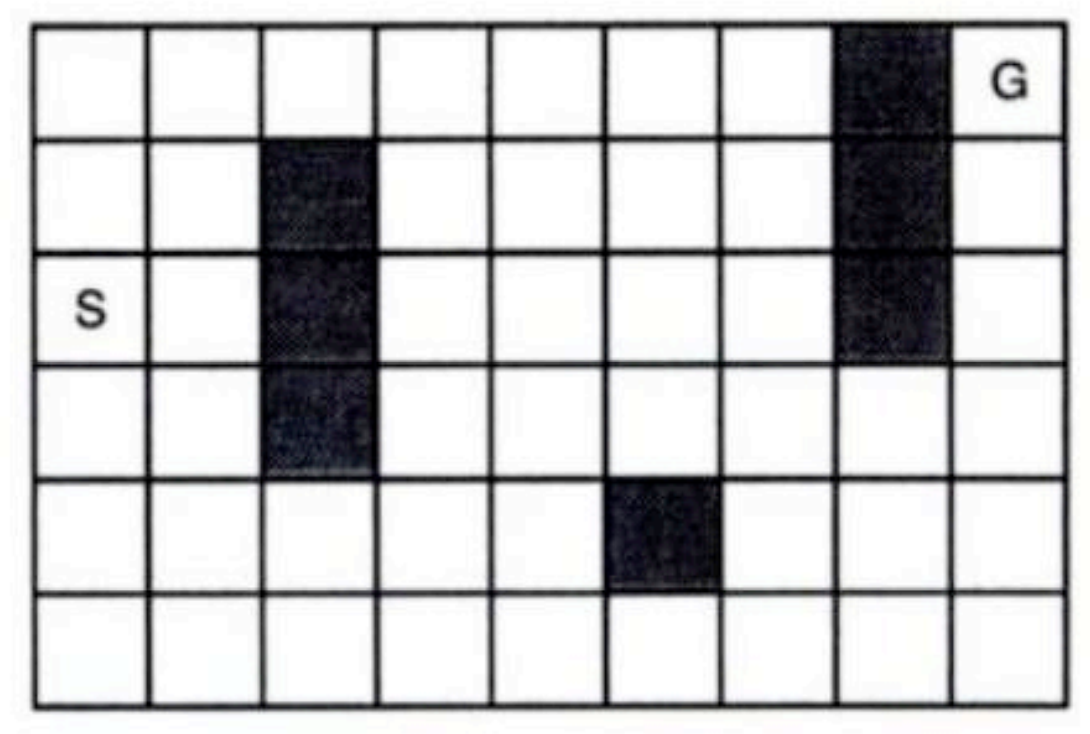
\includegraphics[width=7cm]{dyna}
	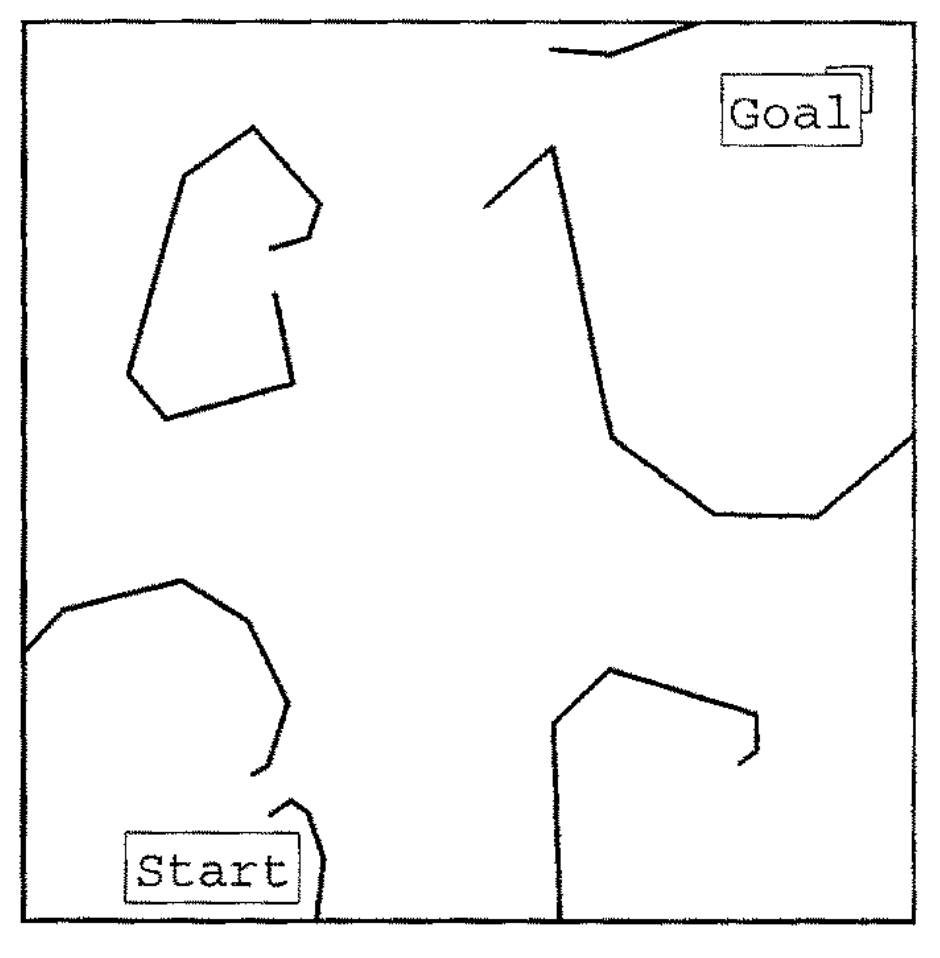
\includegraphics[width=7cm]{parti_game}
	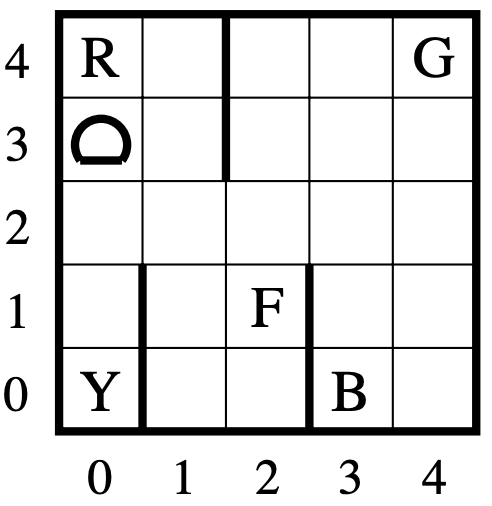
\includegraphics[width=8cm]{maxq}
	\caption{Navigation has always played a central role in reinforcement learning problems. Examples found in Sutton 1990 \cite{dyna} (upper left), Moore and Atkeson 1995 \cite{parti_game} (upper right), Dietterich 1998 \cite{maxq} (bottom) }
	\label{fig:rl_problems}
\end{figure}
Hippocampus has mechanisms that allow it to efficiently (from one or few experiences - similar to one-shot or few-shot deep learning) build maps of the environment \cite{PredictivePlaceCell,space_in_the_brain,model_of_spatial_and_episodic_memory,coding_of_space_and_time}. Dentate gyrus provides pattern separation\cite{Pattern_separation} (effectively preventing catastrophic forgetting). Neuroscientists have also long been speculating that human capabilities of abstract thinking arise from navigation of idea-maps built by neocortex but stored and retrieved by the hippocampus\cite{hippocampal_indexing_theory,Geometry_of_abstract}. 

This yields the hypothesis (formulated by many scientists before) that maps and maximum-reward gradient are two sides of one coin. Maps are fast to build but slower to navigate, policy is slow to learn but fast to use. This paper focuses on the map-building aspect of reinforcement learning. 

Instead of reward, this model introduces the concept of energy. 
The exploration-exploitation dilemma is solved as follows. The agent will
pursue exploration only if it has sufficient excess of energy (according to some threshold). Otherwise the agent will strive to recover its depleted levels of energy by exploiting currently available sources. This is analogical mechanism to hunger among biological organisms. Hence we refer to this as `hunger' signal. According to this definition, reward is received at the moment when hunger decreases. Reward is the derivative of energy. Expected return is defined as sum (integral) of future rewards. Maximisation of expected return coincides with replenishing agent's energy reserves because energy is the integral of reward.  The problem of finding the trajectory with highest rewards is equivalent to search for sources of energy on some map. In this way, we have reduced reinforcement learning to a map navigation problem.

Such definition applies well to certain biological observations. Animals always tend to choose the shortest path leading to their destinations. Shorter distance means less energy is lost on locomotion. Contrary to deep reinforcement learning, where explorations is usually based on random choice of actions with epsilon probability, having an internal map and episodic memory means that agents always know, which areas have already been explored and which are yet unknown.  


\section{Hierarchical Temporal Memory} 

This architecture is primarily based on HTM\cite{bami} networks, although we add three new important mechanisms. Those are pattern separation, voting and polychronization. 

Pattern separation is a property of dentate gyrus, which takes as input very similar patterns and produces new output with much less overlap among the neuronal populations. In reinforcement learning this feature could allow the agent to differentiate between similar situations. For example eating most frogs might be safe but those with red stripes under their eyes might be poisonous and should be avoided. Figure \ref{fig:pattern_sep} presents a graphical illustration of this phenomenon. 


\begin{figure}[!htbp]
	\centering
	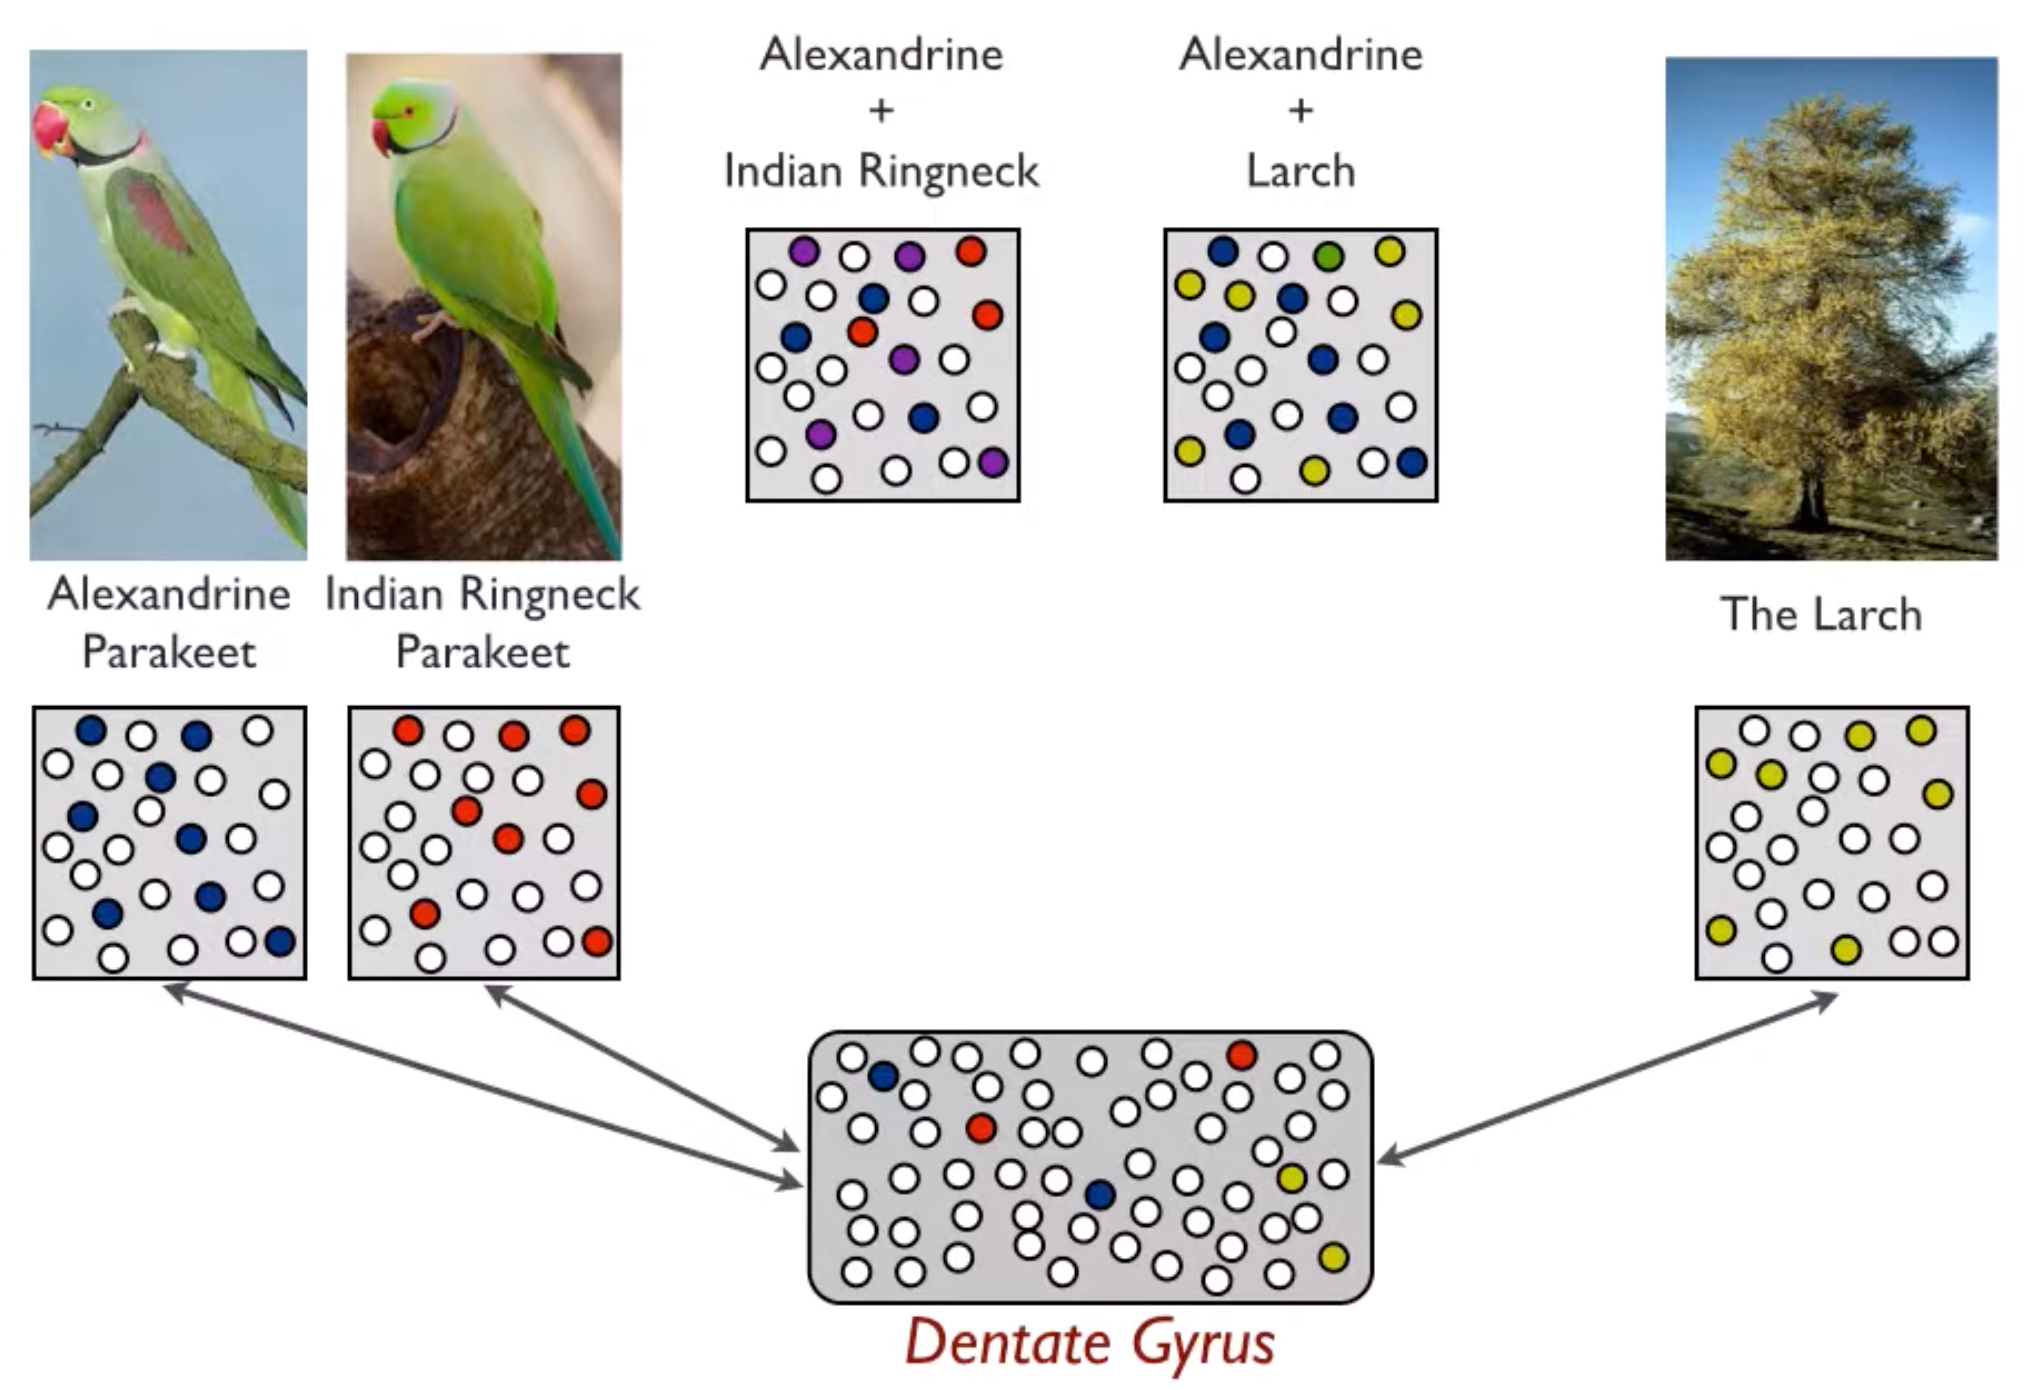
\includegraphics[width=10cm]{pattern_sep}
	\caption{A bird and a tree are easy to tell apart and their internal representation in the network will likely produce non-overlapping activation patterns. Finding a difference between different similar species is a greater challenge. A typical neural network would need to be specifically trained to produce distinct embeddings, but our brains use dentate gyrus to solve this problem much more efficiently. Graphics from \cite{pattern_sep}.}
	\label{fig:pattern_sep}
\end{figure}

The effects of pattern separation are measured as the average overlap in pairs of input and output patterns. It can be reproduced by spacial pooler\cite{spacial_pooler} if the learning is disabled (increment and decrement constants are zero) and the size of output layer is increased. Figure \ref{fig:dg_pattern_sep} compares experimental results in biological brain and in a simulated HTM network.



 \begin{figure}[!htbp]
 	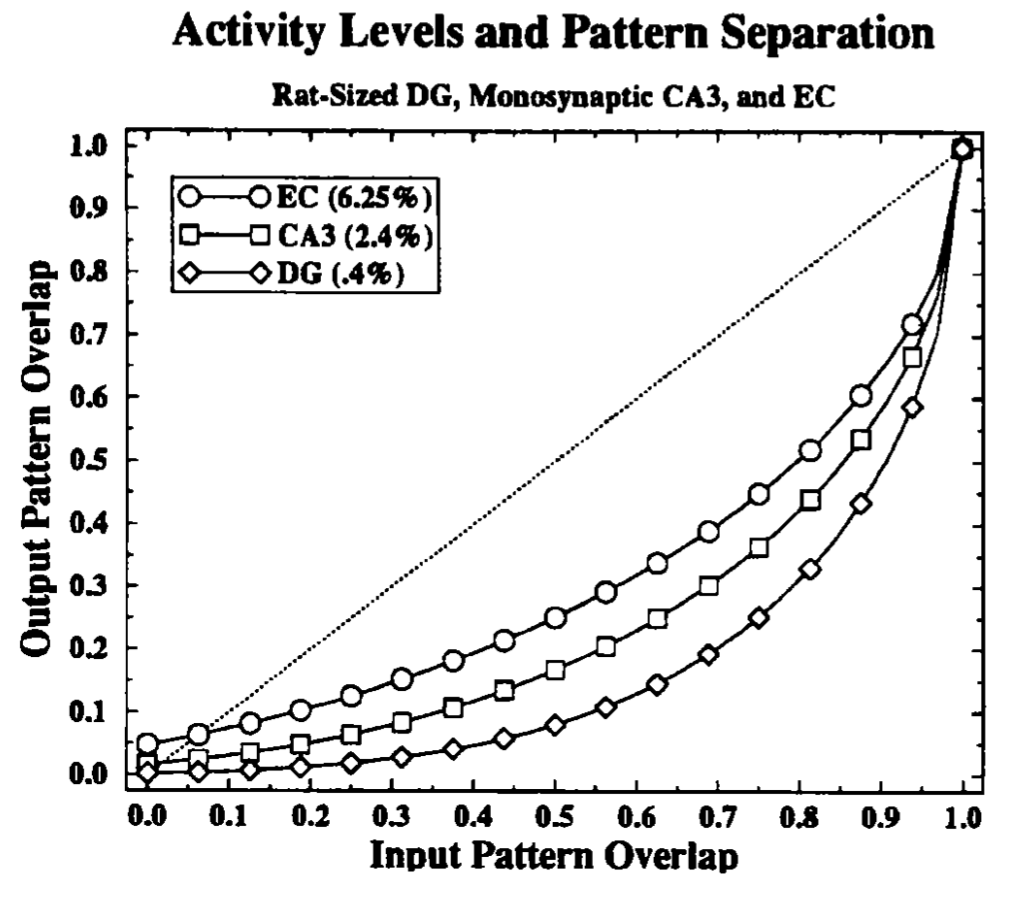
\includegraphics[width=7cm]{dg_pattern_sep}
   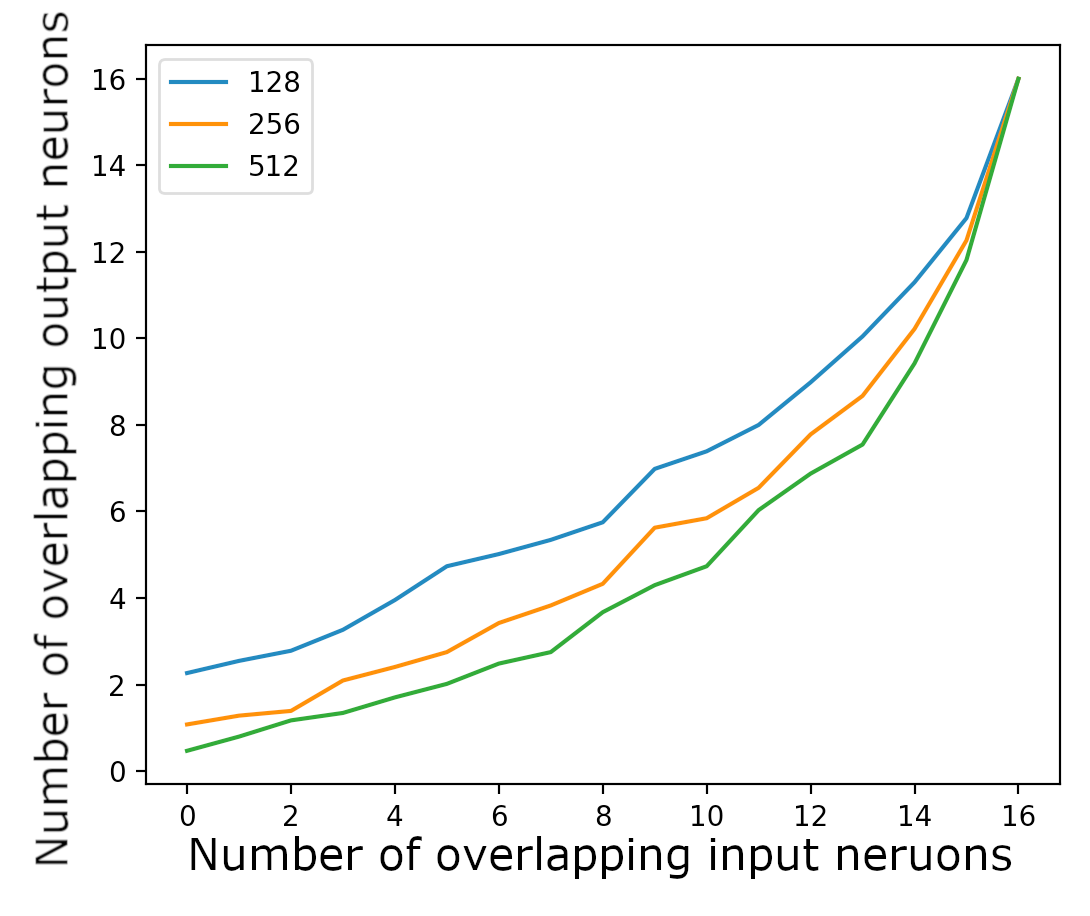
\includegraphics[width=7cm]{exp_pattern_sep}
 	\caption{Left: Empirical approximation of the effects of pattern separation in dentate gyrus (DG), entorhinal cortex (EC) and hippocampal area CA3. Data taken from \cite{dg_pattern_sep}. Right: Experimental benchmarks of pattern separation in spacial pooler with input layer of size 128 and output layer of respective sizes 128, 256 and 512. In these experiments random populations of 16 input neurons were generated. Spacial pooler's sparsity has been configured to always choose 16 most active output neurons.}
 	\label{fig:dg_pattern_sep}
 \end{figure}


Another property crucial for understanding the architecture is voting. To explain it, first let's consider the task of classification. In the standard deep learning setting, a network will receive some inputs and then have softmax output layer that classifies  the data and assigns some label. A spacial pooler could be used in an analogical way. Labels could be encoded as categorical data\cite{bami, Encoding_Data_for_HTM} (subdivide a network into $n$ parts, one for each label and then activate neurons in only one part corresponding to the current label). The input receives some sparsely encoded data and spacial pooler will activate some output population of neurons. To determine the prediction made by network, choose the label that has the largest overlap with currently active output (this is analogical to softmax function). In order to learn the labels, it is enough to increment connections to those active neurons that did overlap with the correct label. In the biological networks it would be equivalent to apical feedback (the correct label) partially depolarizing the output cell. 

The above supervised learning example was simple but consider what happens in the case of unsupervised learning. This means that instead of modelling probability $P(label|input)$, we build a network that sees both label and input. The we train it to model joint probability $P(label, input)$. This scenario also has an analogy in HTM networks. This time we have two columns, each one receiving different input. The first one might see
patch of pixels, a range of audio frequencies, a few scalar values or any other piece of information. The other column might have access to the label. We could then add distal connections from output of first column to output of the other and use patterns produced by one to predict the other. First compute output of column A, then use distal connections from A to B in order to activate B. Next compute output of B based on its input and compare with the activity anticipated by distal connections. Such process could be repeated for both columns and train one from the other in an unsupervised way. This could be generalised further and both columns could be reading different inputs, rather than labels but the fundamental idea is to use activation patterns of different columns as if they were labels.

It is possible to combine both supervised and unsupervised methods into one. There could be distal input coming from neighbouring columns and apical input from above. The most unintuitive and difficult problem is how to generate the apical feedback. We propose an interesting solution. The key insight is that our brains evolved in an environment that is time-consistent. When the observed inputs evolve slowly over time, then if we use activity patterns from previous time step we have high probability of still being correct and up-to-date. What's what we call `sticky' layers. We could compute activations of higher columns once and then use them as apical input in all subsequent steps until something significant happens that forces the higher columns to update. If we have multiple lower columns all connected to the same higher column, then we could put threshold on how many lower columns must agree together in order to overwrite a higher column in case of disagreement. Until there is enough consensus in lower parts, the higher levels do not change. If nobody agrees with anyone and the consensus threshold is not reached, then the higher layers take precedence and their activity is used as labels for the lower ones.
Lastly it should be noted that the higher columns can be initialized randomly at the beginning. If the environment is time-consistent then the system will always settle on some consensus in a self-organizing manner after enough time steps.


The last newly introduced property is polychronization. The real neurons are highly sensitive to precise timing between spikes. The dendrites themselves are time-delayed.
The impulses do not travel at equal speeds through all connections. Polychronization allows
the neural networks to avoid superposition catastrophe \cite{Polychronization}. We do not use continuous-time simulations of neural networks. Instead we reduce polychronization to its discrete-time equivalent. This can be achieved if we use several spacial pooler that consecutively operate on the same SDR. Each consecutive invocation has access to all the original input but it also sees the output produced by all previous spacial poolers. To be more precise define an SDR consisting of $(n+1)m$ neurons and $n$ spacial poolers $S_1,S_2,...S_n$, each one producing output SDR of size $m$. The polychronization is simulated by first writing input to the subregion of
$1...m$ neurons. We restrict $S_1$ to only form connections to that subregion. We run $S_1$ and then copy its output to the subregion $m+1...2m$. Then we run $S_2$, which we restrict to only form connection to the subregion $1...2m$. We repeat the process for $S_3..S_n$. Such mechanism allows each subsequent spacial pooler to be sensitive to the past history of activations in previous layers.  


\section{End-to-end model A} 
The architecture is inspired by the biological brain, albeit much smaller and more simplified. The most significant novelty is that it is the first end-to-end model of the brain.  It consists of 3 layers and a map unit. Those layers are vaguely related to their respective biological equivalents.
This correspondence should be taken with a grain of salt, as the goal of this architecture is not to focus on any specific biological brain, but rather to identify the universal mechanisms underlying all key functions. It should be expected that this model is one of many possible architectures and future research will explore more alternatives, regardless of how similar they are to the real brain.
 
\ctikzfig{architecture A}

The sensory inputs come from many modalities like vision, hearing or touch. This part of the network is typically either evolved using population-based algorithms or designed manually. It might also be possible to substitute it with deep neural networks trained with backpropagation, although this area requires more research. 

The input arrives at the first layer, which was primarily inspired by the neocortex. It consists of one large spacial pooler. It's task is to extract key information from the input and prepare it for voting in the next layer.

The second layer is another spacial pooler whose task is to build representation of agent's immediate surroundings.  Those neuronal populations encode features on a sphere (Figure \ref{fig:rodent_in_sphere}).  It has been largely inspired by the entorhinal cortex, which contains grid cells, head-direction cells and other spacial features. We argue that the grid cells\cite{Recurrent_grid,orientation_sensitive_cells,neural_basis_of_the_cognitive_map} themselves do not play any role in formation of place cells. The visual, auditory and olfactory cues are sufficient and crucial for building maps of surroundings \cite{boundary_vector_cells}. Our model gives new perspective on the true role of grid cells.


\begin{figure}[!h]
	\centering
	
\includegraphics[width=7cm]{rodent_in_sphere}
	\caption{The second layer is topologically equivalent to a sphere surrounding the agent. Each point on its surface contains information about distance and label of a visible object. Hence it forms both a depth-map and outlines of all objects.}
	\label{fig:rodent_in_sphere}
\end{figure}

The sensory input that is received by the network contains information about distance. This is the reason why all animals have two eyes and two ears. By comparing the view from one eye with the other or the sound delay in one ear against the other, they receive information about position in space (some, like birds, don't have stereoscopic vision and they bob their heads instead). This information is crucial and must be preserved by the networks processing the sensory inputs \cite{Object_vector_coding, Neuronal_vector_coding_in_spatial_cognition}.  The first layer (neocortex) will build internal representations of objects at their respective locations. Then all perception will be mapped onto the sphere and locations that end up close to each other on the sphere will clash (there might be less storage capacity on the sphere than there is in the layer 1). In order to resolve these clashes, some voting mechanism is necessary. This voting occurs not only across space but also time. The labels attached to each location are `sticky'. The network has many attractor states and in order to change the label, there must be enough signal coming from outside to knock the network out of its current stationary point. This is a useful property because the real environment tends to be consistent across time. Usually most objects don't move and when they do, the location at next time step is close to the location from previous one. Hence we can use labels from last time step to train layer 1 in the next step. This introduces an (apical) feedback input from layer 2 to 1.
This mechanism of time-delayed self-training is very common and we will also use it again later to train the map.
Because the labels are `sticky', they will remain intact when the agent looks in another direction. Hence it will be aware that the objects do not disappear and are still there even though they are not visible. The sphere itself is the simplest geometrical object that is sufficient to make the layer 2 work, although in biological networks it might be a more irregular shape. The depth-map on a sphere is not well suited to represent concave environments. A ball instead of a sphere might work better. Modifications to the current mechanism will likely be explored in the future, but the current one is the simplest that suffices. 

Layer 3 exhibits the least plasticity and does learn any internal model itself. Its sole task is to facilitate pattern separation. It is much larger than the previous layers. In biological brains it corresponds to dentate gyrus, which is known for being the area most densely populated with neurons. It is implemented as a spacial pooler with low or zero plasticity and a significantly sparser activation. It receives input about the immediate environment and turns it into unique fingerprints that will later be used as the basis for episodic memory.  The connections between layer 2 and 3 have a special property of invariance but in order to explain it, we must first go back to layer 1. As the agent moves its head around the locations of features must rotate along with it, but the output of layer 3 should remain rotation invariant. This could be better explained with a simplified example in two dimensions, using circle instead of a sphere (Figure \ref{fig:rodent_in_circle}). 

\begin{figure}[!h]
	\centering
	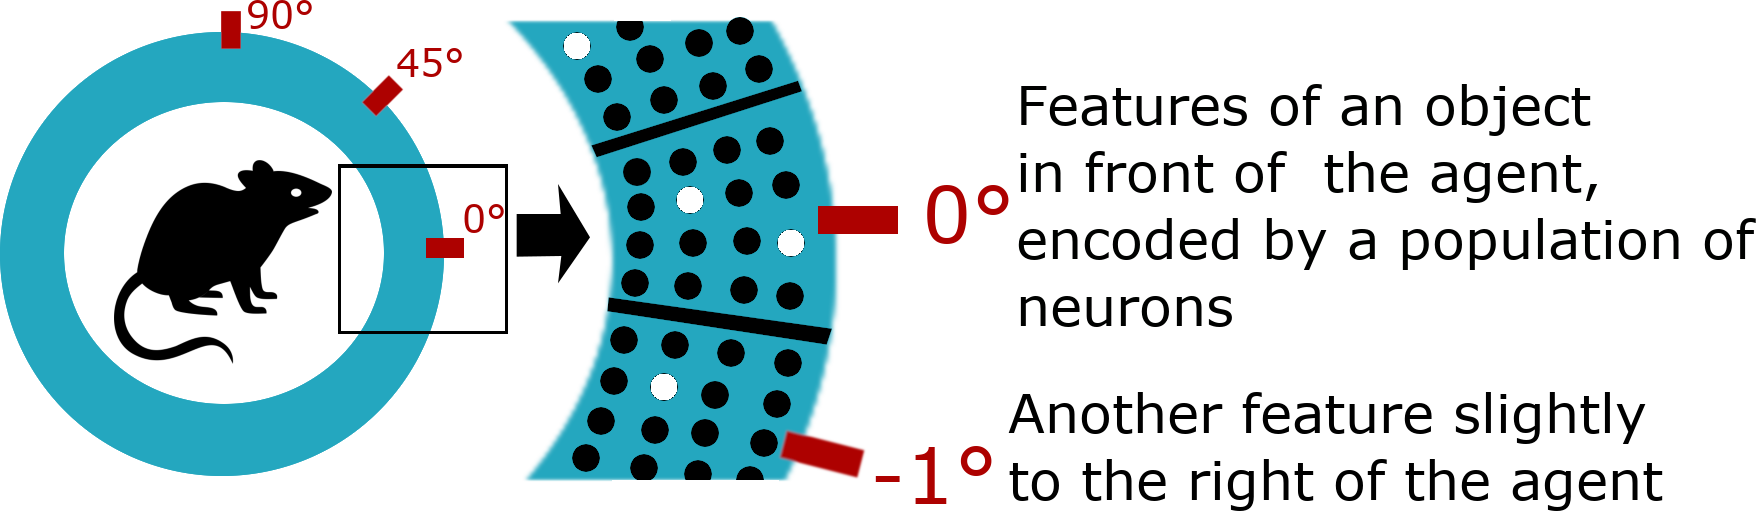
\includegraphics[width=11cm]{rodent_in_cirle}
	\caption{Layer 3 topologically equivalent to a circle contains features of objects in the immediate environment of the agent}
	\label{fig:rodent_in_circle}
\end{figure}

The circle is subdivided into segments containing neuronal populations. Each one of them encodes features of some object visible to the agent at a different angle. Those angles are defined relative to agent's head direction. It is necessary, because the inputs incoming from layer 1 are all  defined relative to the head. The information where objects are located is not encoded by neuronal populations but rather by the topology of connectivity patterns in sensory networks as well as layer 1. Similar ideas were explored  \cite{Locations_in_the_Neocortex}, but the key insight here is that a single column only holds features that appear in very close vicinity and then columns located near each other vote together. This model makes one simplification and assumes that eyes cannot move freely, but rather the view angle depends solely on head position. Hence a specific neuron of layer 1 will fine only if a feature has been detected at a specific angle relative to the head. As the agent rotates its head, the `sticky' populations on the sphere of layer 2 could become misaligned with subsequent inputs from layer 1. In order to ensure that the internal representation does not become detached from the real world, this model will use feedback from motor units to decide when to shift its neuronal populations on the sphere. For example if the agent decides to move its head 1° to the right, then the activity pattern at current -1° population will move to  0°. Pattern from  0° will move to  1° and so on. The important part is that the agent already anticipates the rotation even before motor units perform the desired movement. Then in the next time step the motor movement will be executed and layer 1 will contain information about cues at slightly shifted locations. If the sphere of layer 2 performs its rotation correctly, then the new input from cues in layer 1 will be perfectly aligned with anticipated activity pattern in layer 2. 

Such rotation of neuronal populations gives rise to an emergent property of transfer-learning among distant cortical columns. The feature labels in layer 2 are sticky and rotation will cause them to be reused among different columns over time. For example suppose the agent sees a feature $X$ at 0° angle and this information gets recorded onto layer 2 in form of `sticky' neuronal population. Then the agent turns its head around -45° and the same feature becomes visible to cortical column receiving view from 45° angle but suppose that this column has different connectivity pattern and the spacial pooler produces different output. Layer 2 will move the neuronal population from angle 0° to 45° and the exact same pattern will now be used to train layer 1 column at 45°. As the agent moves around and explores the environment, this process will over time lead distant columns to synchronize together.

It is possible that in the biological brains a process like this might be taking place. Neuroscientists have long observed presence of grid cells and head direction cells. 
Could it be that all this time what we've been seeing were shadows of this more general process of rotation and translations driven by motor feedback?

The final step in building a model of the immediate environment is to design connections between layer 2 and 3 in such a way that makes them rotation invariant. This could be achieved by repeating the same connection pattern for all possible angles (Figure \ref{fig:rotation_invariant_pattern}). 

\begin{figure}[!h]
	\centering
	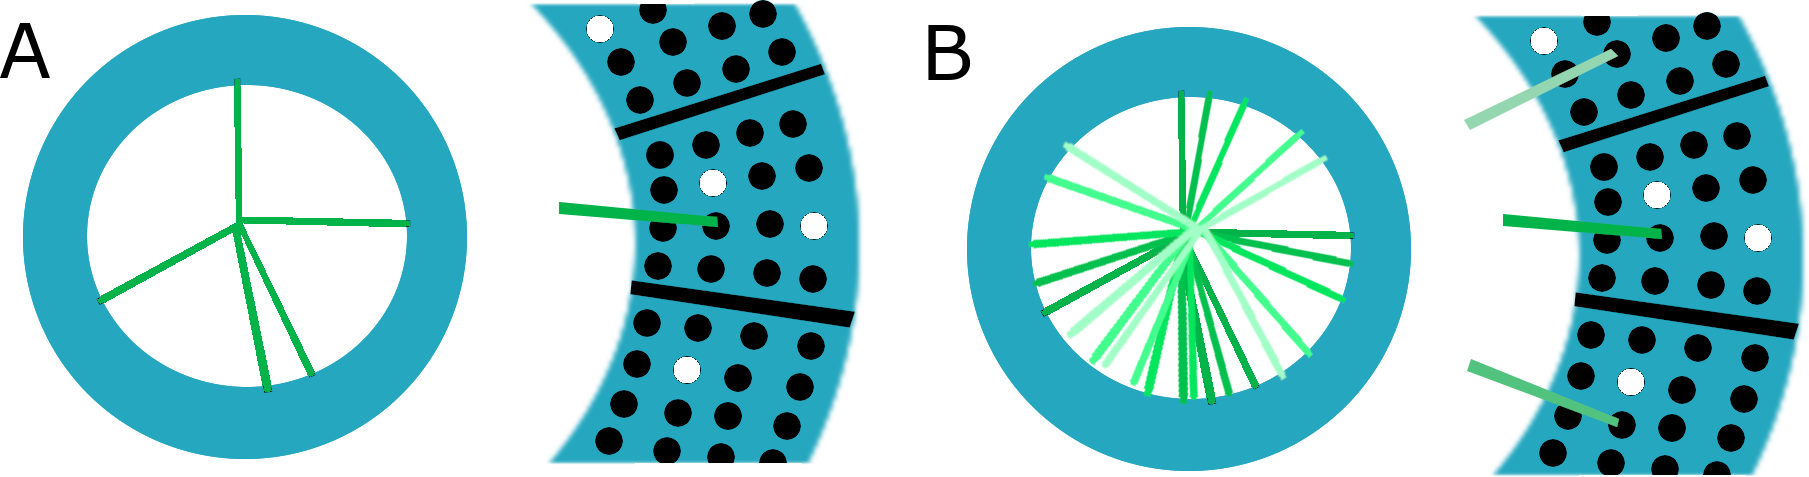
\includegraphics[width=11cm]{rotation_invariant_pattern}
	\caption{Left: a single dendritic segment implementing some connectivity pattern. Right:
	 the same segment repeated for each rotation. The postsynaptic cell will fire if any of the
    segments recognizes the pattern.}
	\label{fig:rotation_invariant_pattern}
\end{figure}


In HTM networks it is implemented by repeating the same dendritic segment for each rotation. If the connections were plastic, then there would be a risk that over time the segments would rewire themselves and diverge from the original pattern. What a coincidence that pattern separation works best when plasticity is disabled. It also has some 
analogies to biological brains. Dentate gyrus has highly organized lamellar structure, suggesting that regularity of connections might be crucial and could facilitate implementation of mechanisms similar to this model \cite{Spatial_Representations_of_Granule_Cells,Pattern_separation_of_spiketrains}. Even if it turned out that layer 2 is not a sphere but rather a more complex shape, dentate gyrus might express various invariant properties in those different geometries. It should be stressed that regardless of how biological this model might be, the invariance mechanisms used here were mostly driven by necessity rather than any explicit attempt at being biologically plausible. 


The most important component of this model is the map. Similarly to layer 2, the neuronal activations here are also sticky. A population of active neurons does not change no matter what input comes from layer 3. The only possible way to update the activity pattern in the map is when the agent changes location in the environment. Until this happens, the currently active neurons are used as `labels' for training connections between layer 3 and the map. Each time a new observation of the environment comes in, passes through layer 2 and causes some new activity in layer 3, we associate that new activity with currently active cells in the map and strengthen the connections between them. The plasticity is modulated by currently received reward. If the agent finds source of energy that decreased its hunger, the reward will be high and the plasticity will be much stronger. When the agent decides that it's time to move and changes its location, the map will change its activity pattern (take input from layer 3 compute output on map as for a standard spacial pooler). Within the map itself there are also many recurrent contextual connections. Their implementation is similar to the temporal memory algorithm\cite{htm_sequence_learning} in HTM networks. If the agent finds itself in the same spot it will be able to imagine and plan future trajectories by following those strengthened recurrent connections \cite{future-paths}. The plasticity again depends on reward.
When an agent stops at point $X_0$, then takes actions $a_1, a_1, a_2... a_n$ to traverse through locations $X_1, X_2, X_3,...X_n$ and the finally stops as location $X_n$, the path of recurrent connections corresponding to transitions  $(X_0,a_1)\rightarrow X_1$, $(X_1,a_2)\rightarrow X_2$ ... and so on, will be strengthened. Depending on whether $X_n$ contained a reward or not, the plasticity will be different but some strengthening will always take place. For a single trajectory, it is necessary to perform the strengthening in several iterations. As long as the agent remains idle at state $X_n$, the map will keep replaying the last trajectory and strengthening it. With each subsequent replay, it will omit certain intermediate steps. This allows for the effect called time compression. As a result, next time agent finds itself in the same spot $X_0$, it will be able to plan future trajectories in stepping stones, rather than individually  action by action. This allows agent's imagination to efficiently make plans running far into the future. The stepping stones usually will be the idle states like $X_0$ or $X_n$ and the intermediate states will slowly fade out of the memory over time. If the agent then decides to continue walking and reaches  a third idle state $X_m$, then during planning the agent will hop through sequence $X_0\rightarrow X_n \rightarrow X_m$. During execution of the plan, the agent will find itself first at state $X_0$ and its goal will be to reach $X_n$, however there will be no state-action pair in its memory corresponding to $(X_0, a)\rightarrow X_1$. Instead there will be a memory of $(X_0,a_1)\rightarrow X_2$ and this will be chosen. If over time it turns out that the agent frequently traverses trajectory $X_0...X_n...X_m$, it might start forming a routine. It will less often stop at $X_n$. Instead most of the time it will start executing trajectory $X_n...X_m$ immediately. As a result, no stops will be made at $X_n$ and it will slowly fade out of memory as well. In the end the agent will only remember  the stepping stones $X_0...X_m$. This is the mechanism by which the less important stepping stones are dropped from the memory and only the important fragments of each episode are retained. Biologically this mechanism corresponds to the episodic memory of hippocampus \cite{Temporal_binding}. The neurons active in the map correspond to place cells, which fire only when animal finds itself in a specific location. 

The final layer contains neuronal populations encoding actions and we refer to them as motor units on the diagram.  They implement the mechanism responsible for updating place cell activity. The model will continuously alternate between map and motor units 
and update the respective patterns in a loop, ignoring of input incoming from layer 3.
The connections between those layers are implemented as two spacial poolers. If the agent is idle and doesn't do much, then activity among motor units will be too sparse to update the sticky activations in the map. It might be possible to run the system in two independent threads. One thread computes the sensory inputs going through layer 1, 2 and 3. The other computes activations on the map and motor units in an infinite loop. Such a busy loop would cost a lot of energy. In order to save unnecessary computation, the second thread might update only when the motor feedback arrives. If the agent moves faster, then the map activity will be updated more frequently. If it moves slowly or not at all, then the map will update less often or remain unchanged.

The exact recipe for implementing the loop requires polychronization mechanism.
Consider the map to be the first layer and motor units to be the second. We use spacial pooler that can see both the map and the activity of motor neurons. Using those two inputs it then tries to infer the next activity pattern on the map. This corresponds to modelling the the transition $S \times A \rightarrow S$ in `standard' reinforcement learning. The above mechanism may seem like an overly complex description of a simple spacial pooler. If we used continuous-time neural networks, the polychronization mechanism could give rise to complex motor synchronization and would allow for encoding of continuous time and distance. Because we are using discrete time-steps, it reduces to a simple special case of a single spacial pooler.

For a long time neuroscience was not able to explain the exact mechanisms responsible for formation of place cells. This paper is the first one to give this explanation in form of a precise algorithm. This model is biologically plausible. It has been observed that the brain activity of idle animals
is very different from the actively moving ones \cite{swr_correct_and_error}. The alternation between map and motor units corresponds to the theta cycle. It has been observed that frequency of theta cycle changes in proportion to speed of moving animals. During idle states, hippocampus often experiences sharp-wave-ripple events, which replay the recent experience in reverse order. This model does not require to perform the replay in reverse. It might be a necessary mechanism for biological neurons, but a computer algorithm might as well temporarily store the sequence of actions in a data structure. I suspect this should not make a significant difference. Another parallel that could be drawn is the reward system. In biology, the brain will secrete dopamine, which serves the same purpose, but in virtual environment the reward system might be either programmed by hand or fine tuned using evolutionary methods.  

The model also includes a special layer with neuronal activations arranged in a grid-like formation. This layer is optional. The map will be trained correctly without it. The reason why it might be beneficial is due to the nature of spacial navigation. If the agent finds itself at some location $X$ and the planning algorithm decides that the highest reward can be obtained at location $Y$, then the agent without the grid layer will be forced to repeat all the actions stored on the map. Those actions might be suboptimal. For example consider a scenario in which the agent arrived at $X$, then explored the places $A,B,C$ and then ultimately found some reward at $Y$. The next time agent finds itself at $X$ the map will be telling it to go through the sequence $A,B,C$ again, but there might exist a straight-line path leading from $X$ to $Y$ without intermediate states. If the agent could associate specific spacial coordinates to each place cell, then the planning algorithm could make use of such information to always generate straight-line routes. This is the task of the grid layer. Its activation pattern is a simple grid of `sticky' neurons. The only input that can change its activations is the action output and the place cells on the map. The former input takes precedence in novel locations, whereas the latter is used to provide corrective feedback that ensures stability and consistency of the grid for already explored locations.

Lastly this model leaves room for feedback connections from the map to layer 1. This allows for recall of past memories and reliving their experiences. It can be trained in the same way as the connections between the map and layer 3. The real brain uses attention mechanisms to only focus on certain important fragments of the experience, instead of making perfect recordings of the past like a movie. I do not include such mechanisms in order to keep the model simple. Analogically not all actions are equally important. An agent being in an idle state is not frozen in time. It may still perform many minor actions like looking around, sniffing, listening, grooming etc. In the future research we might need better mechanisms to differentiate between important and unimportant actions. In this simple model, such distinction is configured manually.  As of now we suspect that a promising path for implementing attention mechanism is by paying greater attention to variance in neuronal populations, especially in layer 1. If the inputs of the world change too frequently and rarely make meaningful contributions to voting, then it is likely due to aleatory variability. The brain could have evolved mechanisms to inhibit such inputs in order to save energy on unnecessary neuronal activity.

In the biological brains most motor activity is controlled by the neocortex. It's possible that a more complex model than this could make improvements by following a similar path. The planning and choice of action trajectories is also achieved with manually programmed algorithms. It is possible that we are missing some layers that could intelligently perform this process.


\section{Generalisation of model A}

The model described so far has certain shortcomings.  It is impossible to integrate motor feedback with layer 2 and all of the columns in layer 1 must be perfectly synchronized to always produce the same output for the same input. The rotation mechanism in layer 2 could be generalised using mechanism similar to that between the map and motor units. Consider the following scenario
\begin{itemize}
	\item Column X in layer 2  receives sensory input from certain area (let's say SDR U) and produces SDR A in layer 2.
	\item Rotation takes place and SDR U is moved to a different area of sensory neurons. Now this input is received and ends up arriving at column Y in layer 2.
	\item Column Y produces different SDR B for this exact same input SDR U.
	\item Even though SDR A and B may be different, it is not a problem. We can use hebbian learning to associate activations on the motor units and previous SDR A with the new SDR B. This is a generalisation of the rotation mechanism, which does not require all of the columns to be perfectly synchronized.
\end{itemize} 
Even if we could make the above model work in layers 1 and 2, it would fail in layer 3. That's because the rotation invariance can only work when all columns produce the same outputs. If SDR A $\ne$ B then after rotation the pattern A will be replaced by B and the rotation invariance is broken. Hence this model cannot be generalized. All the columns in layers 1 and 2 must be perfectly synchronized, which means that no hebbian learning can occur there. It is also not very biologically plausible, because it would require all cortical columns to be exactly the same and have identical topology of connections  with entorhinal cortex. Moreover the idea that internal representation of immediate environment in layer 2 is a sphere or a ball suggests that we should be able to perfectly imagine our entire surroundings even with our eyes closed. But we can't actually do that. Nobody has 360° panoramic imagination inside their heads. 

Those are the reasons why this model is not only impractical from algorithmic point of view, but also biologically implausible. However... certain ideas presented in this model were going in the right direction. It was almost right. 


\section{End-to-end model B}

This model has many similarities to the previous one but the layer 2 is gone and there is no need for segment repetition in layer 3. The columns in layer 1 no longer need to be synchronized. Voting mechanism may still be used, but it's sole purpose is to extract coarser features from the fine ones. 

To better understand the motivation for this new model, start with a simple thought experiment. Close your eyes and try to imagine your surroundings. Can you see everything at once? Most likely not. Whatever you imagine it is always a view from some specific standpoint. That view may not be very detailed. Usually when you imagine some location, you can either see a vast area but lacking most of fine details. Only once you focus on a specific object, your imagination will produce the finer textures and shapes. We do not see all of our surroundings at once, but instead we use our attention like a spotlight that can shine on a very narrow area. This `spotlight' always shines from a specific location and angle. Hence it works as a `pointer'. It is encoded using grid cells and head direction cells. We can use this pointer to search through our past memories in the hippocampus. They will activate specific place cells. Then the memories could be visualised. The place cells retrigger past experiences. Instead of storing the entire immediate environment at once (like it took place in layer 2 of model A), we only store the pointer (and the motor feedback only needs to update the pointer itself). Then we associate sensory input \textbf{and} the pointer with a specific place cell in the hippocampus. The agent can generate the model of immediate environment  in its imagination by creating a `mock' pointer and then querying the place cells. Hence even though model B does not have layer 2 in the same explicit way as the model A used to, the pointer works as a compressed representation of layer 2. That's why we could say that model B is a compressed and simplified equivalent of model A.

The model B has additional advantage over model B. Because we separate pointer from sensory input, we can easily implement attention mechanism. Connect every sensory modality to the map layer (hippocampus) and then create a `switch' that allows only one modality (or a specific combination of them) to arrive at the same time. Then this switch may also become a part of the pointer, along with head direction and grid cells. This mechanism is very general. It is possible to further enrich the pointer. An additional layer of working memory could be inserted into the network. Such layer could hold short-term auxiliary variables. If the neocortex grows larger, it will have excessive area that has no particular use. Those areas could then reconnected to receive input from somewhere else, which in turn will drive emergence of new auxiliary variables. Some of them might contribute to the pointer and enrich it in a meaningful way. The evolution would favour connections that give rise to meaningful pointer enrichments. 

If the model A was correct, then with the help of layer 2, the agent should be able to imagine the entirety of its surroundings in a panoramic-like vision. Humans do not poses such abilities, except only in one case. Even with our eyes closed, we can always `feel' our distance to all surrounding borders of the environment. The entorhinal cortex is known to contain border cells. Our hypothesis is that the mechanisms similar to that in layer 2 of model A are present in the real brain, but they do not store all information. Instead the layer 2 in model B only keeps track of borders and certain landmark objects. It has also been observed that entorhinal cortex contains vector-object cells. Those neurons can be used to implement vector fields and precisely locate all nearby objects. Such mechanism not only allows for a compressed representation of the original layer 2 but it also provides a reliable way to associate different views of the same object with one and the same place cell in the map layer. 

Imagine you're looking through a spyglass. You also have a lidar to measure distance. If you know your own location and head direction, then you can precisely tell the location of distant objects. Your task is to mark them on a map, but you are not allowed to mark your own location on the said map. Instead you assume that your position is always in the centre and as you move, your location stays constant but the entire map moves instead. This map might be large and physically redrawing it with each step would require a lot of work. So instead of drawing the map with all details, you only select a few landmarks and mark them with dots. Then you keep a reference from each dot (the place cell) to some different sheet of paper  that contains detailed description of the object (population on the neocortex).
Now as you move around, you only need to redraw the dots. When you observe the same location from a different perspective, you look up the right dot, use the reference attached to the dot and follow it to locate the additional sheet of paper with the detailed description of the object and then you use the newly observed experience to enrich and refine that description. The key component of this model is the mechanism allowing you to look up the right dot. To explain it, consider the simplest scenario of a map with only one dot.

The model B:
\begin{itemize}
	\item Receive inputs from sensors and run them through layer 1.
	\item Layer 2 works like a ball. However it does not store features of objects, like it was in model A. It only stores a single bit that specifies whether given location is occupied or not.
	\item Cast layer 1 onto layer 2 in the an analogical way as it was done in model A.
	\item Use grid cells and head direction cells to normalize the layer 2. For this reason layer 2, grid cells and head direction cells must be stable. If they are stable, then it is possible to always use them to normalize the surroundings.
	\item Once the surroundings have been normalized, no rotation invariance is necessary. Hence, the rotation invariance between layer 2 and 3 has been substituted for normalization. Normalization does not need to produce a new layers, but instead it is then directly used to activate place cells. This normalization is a mechanism that is implemented `in dendrites', not `in cell bodies'.
	\item Use the normalized environment together with current head direction and grid cell pattern as part of pointer to the map layer. You need to store them, so that when you see the same cues later, you will restore the same grid and head direction. This will allow for stability of environment representations.
	\item Whenever the agent looks at some object, we can now also normalize the experience. If we know the position of that object, relative to the head, we only need to add the vector of our own location (using grid cells) . We could also store this vector in the memory itself, in order to later recall what the object looked like from a specific point of view.
	\item The agent needs to keep its model of the environment up to date. If something moves, the agent will look at it more closely and update the model. If the exact same movement pattern repeats, the agents will become less sensitive to it. This mechanism of attention is implemented in the thalamus. Novel input triggers some areas on the cortex to respond and those in turn will trigger inhibition in the thalamus, so the attention is only short-lived. 
	\item Certain parts of the environment do not change very often. Such cues make good candidates for landmarks that could be later used to identify the same location. The agent operates two modes of vision. The narrow vision is used to update the novel and moving parts of the environment. The broad vision is used to identify constant landmarks. It is the landmarks that are used to restore grid cells to ensure their stability.
	\item The hippocampus is a `sparse associative map'. This map is capable of abstract thinking, by factoring out common features among many similar inputs.
	This leads to emergence of gnostic cells that encode abstract ideas. Sparse associative maps learn much better when the input is orthogonalised. In model A, all cells on the sphere encoded objects and  their locations jointly. As a result the model would need to relearn the same object at each specific location. In model B, the objects are represented separately to their locations. This way the brain can learn about an object once and then imagine it at any location. Orthogonalisation leads to more efficient maps.
	
\end{itemize}







% \ctikzfig{architecture B}



\section{Navigation is the foundation for general intelligence}

The mechanisms described in this paper could be potentially used to build general human-like artificial intelligence. The neuronal populations that emerge in the map layer 
respond to particular physical places in the environment. If an agent navigates a set of rooms, then inside each room there will be populations that become active in narrow and specific places of those rooms, but there should also exist certain neurons that are shared by all those populations. Such neurons will be more general. They could be used to encode the abstract idea of a room. We speculate that such abstract cells will emerge if instead of a sphere we use ball in the layer 2 and it covers vast enough area. 

It has been observed that brains of primates contain a specific type of place cells that activate when the animal looks at a particular region in space. Those are called spacial-view cells \cite{Spatial_view_cells}. There have also been accounts of place-like cells used for encoding position of limbs \cite{Place_Cell_Like_Activity_in_the_Primary_Sensorimotor}.
An agent that is capable of visualising and manipulating 3 dimensional structures and building maps of them in their imagination, would be capable of generating ever more complex cells of abstract ideas. We speculate that the combination of visual imagination with precise limbic manipulation might lead to emergence of human-like general intelligence. It would allow the internal maps to form abstract ideas of numbers, causal relationships and more. 


\section{Can we derive this architecture mathematically?}

Consider the following necessary properties:

\begin{enumerate}
	\item \label{prop-pop} Assume that all important information is encoded entirely by populations of active neurons. Let's ignore firing-rate and relative timing of spikes. We operate under the assumption that all fundamental algorithms responsible for intelligence in our brains could be expressed on any Turing-complete system. Biological neurons operate in continuous time, because the natural environment and physics are embedded in continuous time, but the algorithm is simple and general enough that it could be reduced to a discrete-time special case and still work correctly.  
	\item \label{prop-place}  The place cells are rotation-invariant
	\item \label{prop-sense}  The sensors are not aware of their position is space but are permanently bound with the body and information about their location with respect to this body is constant.
	\item \label{prop-no-relearn} If you can recognize an object from its tactile features with your left hand, then you don't need to relearn the same sensory inputs in your right hand. If you can see an object with left eye, you can automatically recognize it with the right one. Suppose you are looking at some point in space and the reflection of some object falls onto some specific region in your retina. If you then look at a different point in space and reflection of the same object falls onto a different region on retina and activates different set of photoreceptors, you can still recognize that object.
	\item \label{prop-rot}  If you are aware of the position of walls and other objects in your room and then close your eyes and rotate your head (or entire body), your imagination of the room will still be spacially consistent. The positions of objects are not `frozen'  relative to your head. Your imagination of the room will rotate in the opposite direction to the rotation of your head. The internal representation of the room cannot be rotation-invariant, because then you would not be able to locate anything with your eyes closed. Instead, it must be `rotation-consistent'.
\end{enumerate}

What are the logical implications of the above assumptions?

\begin{itemize}
	\item \ref{prop-sense} and \ref{prop-no-relearn} $\implies$ The layers close to sensory inputs do not hold any information about `labels' or `objects'. A single column in the visual areas of occipital lobe can receive input only from a limited field of view. If it was the case that our brain attempts to perform classification task in those columns, then we would need to train every single column separately. But then you would not be able to recognize the same object with your left eye, if you only experienced it with the right one. Hence  we can deduce that the brain does not perform object classification, at least not using cortical columns. This implies that the "thousand brains theory" and their model of sensorimotor object recognition is wrong. Each cortical column does not build its own representations of any objects. The columns only see features. If there is any hierarchy, then the higher-level columns might be able to see coarser and more general patterns among the features, but they do not convey information about object categories like `cups' and `tea pots'. (There are gnostic cells in temporal lobe that respond to specific objects, but this is true only for primates, whereas all other brains can work without performing such object classification.)
	\item \ref{prop-rot} $\implies$ Representation of the immediate environment must be stored persistently even when no input is coming. It must also be responsive to motor feedback. The stored information should not be degraded (at least in the short term) by sequences of actions that result in no operation. For example rotation in one direction followed by opposite rotation of equal angle results in the same position as there was at the beginning. Whatever transformation was performed on the neuronal populations by the motor feedback, must be invertible. This means that the effect of motor feedback during rotation must work like an invertible function, implying that it is a bijection (or at least a close approximation thereof).
    \item \ref{prop-rot} and \ref{prop-sense} $\implies$ Suppose that the immediate environment is encoded using neuronal populations such that each neuron is active only when some feature has been detected at some position relative to the head. Then as the agent rotates with closed eyes and there is no new input incoming, the internal representation will stay constant relative to the head and it will be out of sync with actual locations of objects. Hence it is necessary that the  neuronal populations themselves rotate. 
\end{itemize}

\bibliographystyle{BibTeXtran}   % (uses file "BibTeXtran.bst")
\bibliography{BibTeXrefs}    







\end{document}
